% -*-latex-*-
%\documentclass[pdftex,handout]{beamer}
\documentclass[pdftex,12pt]{beamer}
\usepackage{etex,pictex}
\usepackage{color}
%\usepackage{pst-plot,color,pstricks}
%\setlength{\topmargin}{-1.7in}
\begin{document}

\title{Detecting Selective Sweeps}
\author{Alan R. Rogers}
\date{\today}

\frame{\titlepage}

\begin{frame}
\frametitle{Outline}
\begin{itemize}
\item Questions
\begin{itemize}
\item Have humans evolved rapidly or slowly during the past 40~kyr?
\item What functional categories of gene have evolved most?
\end{itemize}
\item Selection and recombination
\item Data
\item Results
\end{itemize}
\end{frame}

\begin{frame}
\frametitle{Are we still evolving?}
\begin{itemize}
\item Since split with chimps, there has been
  rapid evolution in proteins expressed in brain and in sperm.
\pause
\item Recent selection at various loci: lactase, DRD4, etc
\pause
\item How common are such loci in the human genome?
\pause
\item How can we tell?
\end{itemize}
\end{frame}

\begin{frame}
\fbox{\includegraphics[height=0.9\textheight]{sweep-chswrth.png}}
\end{frame}

\begin{frame}
\begin{columns}
\column{0.6\textwidth}
 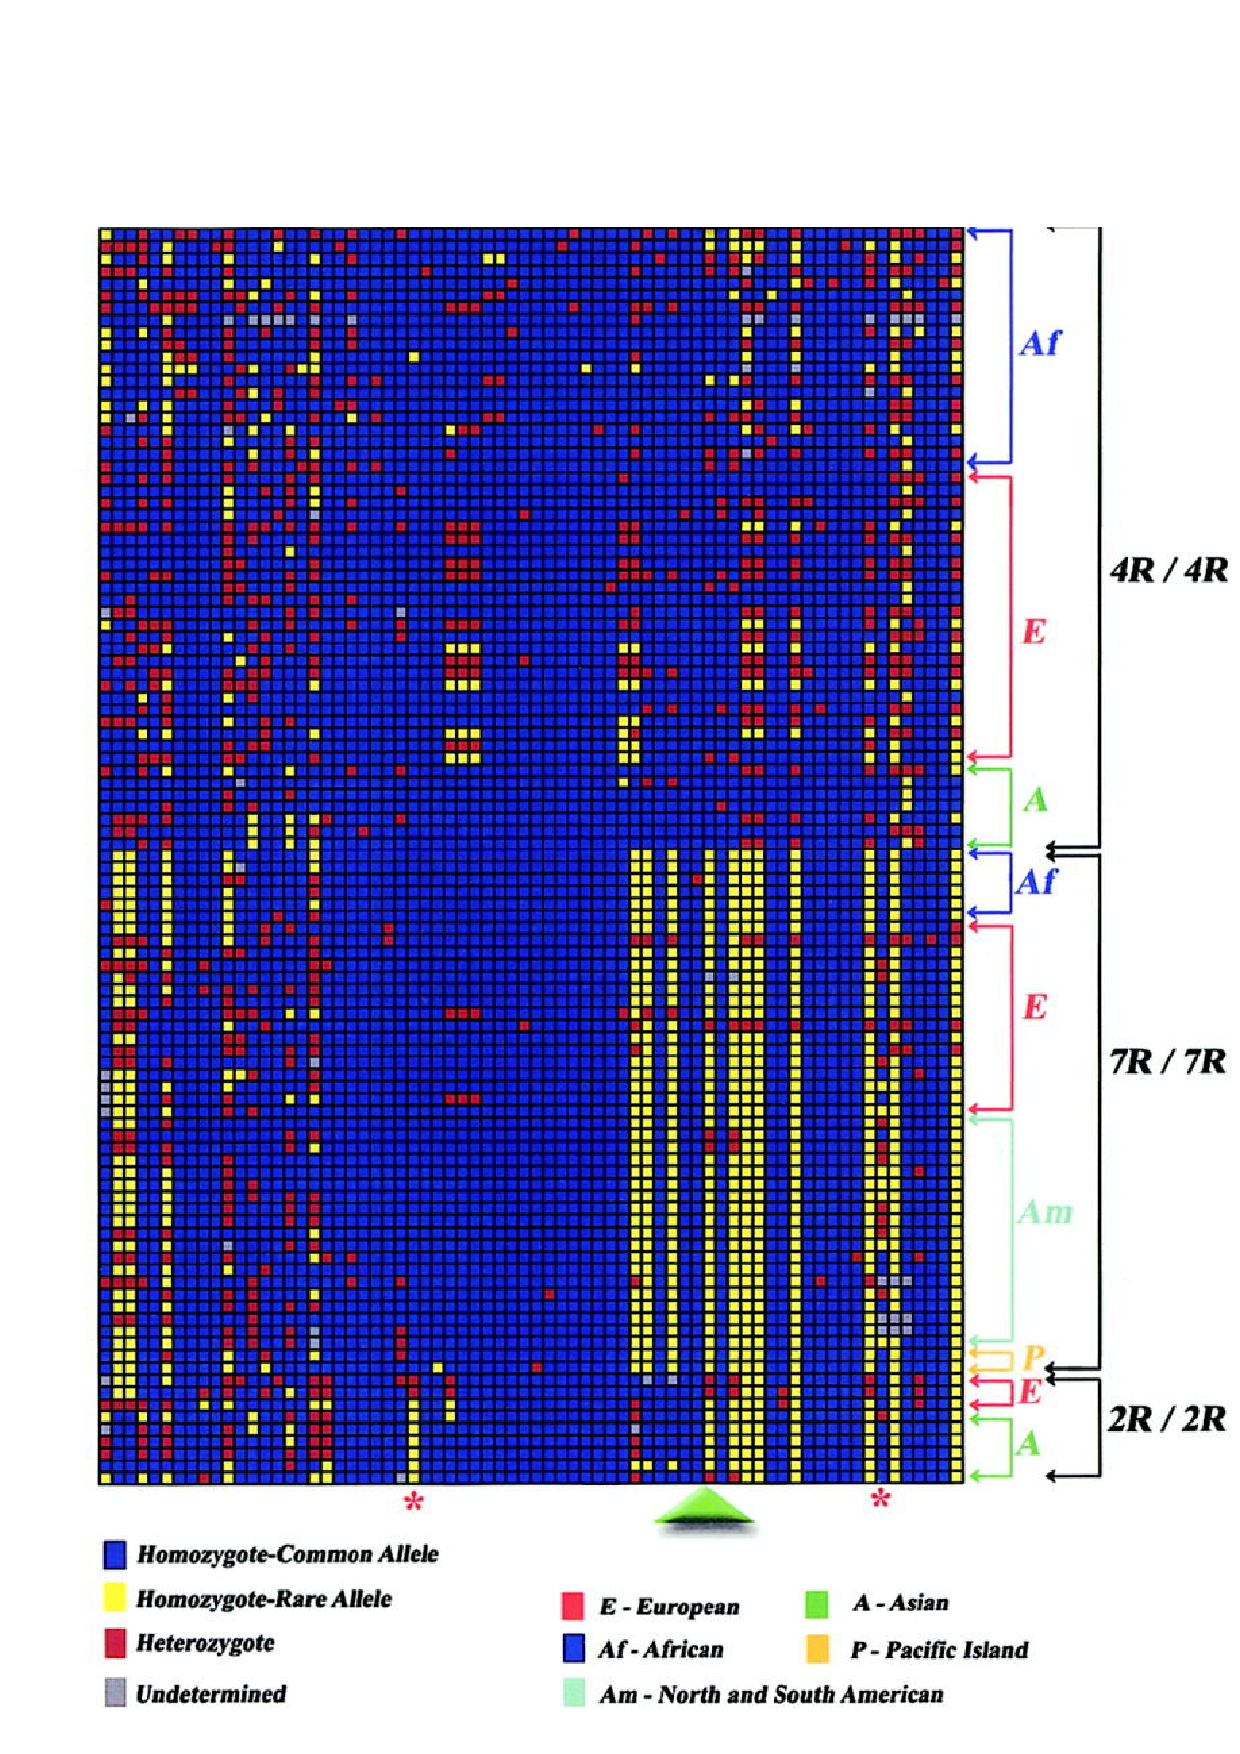
\includegraphics[width=\textwidth]{drd4-polymorph.pdf}
\column{0.4\textwidth}
\raggedright
Signature of an ongoing selective sweep at DRD4
\begin{itemize}
\item Sweeping allele is
\begin{itemize}
\item common
\pause
\item has low diversity over large region
\end{itemize}
\pause
\item High LD over large region
\end{itemize}
\end{columns}
\end{frame}

\begin{frame}
\frametitle{Finding sweeping alleles}
\begin{itemize}
\item Extended haplotype homozygosity (EHH): Voight et al 2006
\end{itemize}
\end{frame}

\begin{frame}
\frametitle{Idea behind Extended Haplotype Homozygosity (EHH)}
\begin{columns}
\column{0.5\textwidth}
%DNA sequences near human lactase gene, typed in a
%European sample.  Columns are
%nucleotide sites.  Top row (the
%reference sequence) shows common state at each site. Capital
%\texttt{A} is lactase persistance
%allele\cite{Bersaglieri:AJH-74-1111}.  Numbered rows represent
%individual chromosomes. Dots indicate identity with top row.  60
%chromosomes identical to reference sequence were omitted to save
%space. From HapMap release r23.}\label{tab.lctseq}
%
\tiny
\centering
\ttfamily
\begin{tabular}{c@{\hspace{1.5ex}}c}
  &ctaaacagaccaacgtaAgggtacaatgcctaacccagacgttt\\
20&............................................\\
21&............................................\\
22&............................................\\
23&............................................\\
24&............................................\\
25&............................................\\
26&............................................\\
27&t...........................................\\
28&t...........................................\\
29&................................c...........\\
37&.................G..a.gt.....t.........gac.c\\
38&t..gg..c.....tc.gGaaa.g..ccttt...tg......c..\\
39&t..gg..c.....tc.gGaaa.g..ccttt...tg......c..\\
40&t..g.....t..ttccgG..a.gt.....t.........gac.c\\
41&t..g.....t.gttccgG..a.gt.....t.........gac.c\\
44&t..g.....t..ttc.gG..acgt.....t.........gac.c\\
45&t..g.....t.gttc.gG..a.gt.....t.........gac.c\\
46&t..gg..c.....tc.gGaaa.g..ccttt...tg......cg.\\
47&t..g.....t.gttccgG..a.gt.....t.........gac.c\\
48&t..g.....t.gttccgG..a.gt.....t.........gac.c\\
49&t..g.....t.gttccgG..a.gt.....t.........gac.c\\
50&tcgg.tc.g.tg.tc.gG..a.g.g....tg....ggt...cg.\\
51&tcgg.tc.g.tg.tc.gG..a.g.g....tg....ggt...cg.\\
\end{tabular}

\column{0.55\textwidth}
\textcolor{blue}{Upper half:} pairs of chromosomes are identical
at most sites

\bigskip\pause

\textcolor{blue}{Lower half:} pairs identical at fewer sites

\bigskip\pause

This idea underlies EHH.
\end{columns}
\end{frame}

\begin{frame}
\frametitle{Study of Voight et al (2006)}
\begin{itemize}
\item 800,000 SNPs in 309 people
\item 431 sweeping loci
\item Most sweeps started w/i past 10,000 years
\end{itemize}
\end{frame}

\begin{frame}
\begin{columns}
\column{0.65\textwidth}
 \includegraphics[height=0.9\textheight]{voight-venn.png}
\column{0.35\textwidth}
Voight et al (2006): 431 sweeping loci.

\medskip

{\color{red} ASN: Asia\\
\color{green} YRI: Africa\\
\color{blue} CEU: Europe.}

\medskip

\pause
Most are sweeping w/i only one continent.

\pause
Also true of Wang et al data.
\end{columns}
\end{frame}


\begin{frame}
\frametitle{Diversity trough around exons in
  \textcolor{green}{\textsc{yri}}, 
  \textcolor{red}{\textsc{ceu}}, and
  \textcolor{blue}{\textsc{chb+jpt}}} 
{\centering
\includegraphics[height=0.8\textheight]{Hernandez-trough.jpg}\\}
\end{frame}

\begin{frame}
\frametitle{Selective sweep predicts a trough in diversity}
\includegraphics[width=\textwidth]{JHG_fig4_4.jpg}
\end{frame}

\begin{frame}
\frametitle{Why the trough?}
As the favored allele sweeps to fixation, alleles at linked loci
`hitch-hike'' to higher frequency.

\bigskip

Reduces diversity at linked loci.

\bigskip

Effect declines with distance from sweeping site.
\end{frame}

\begin{frame}
\frametitle{Purifying selection also predicts a diversity trough}

Mildly deleterious mutations may drift to moderate frequencies.

\bigskip

Are eventually removed by selection.

\bigskip

Any mutations at linked sites are also removed, lowering diversity at
linked sites. This is called ``background selection,'' as Jon will
soon explain.
\end{frame}

\begin{frame}
\frametitle{Hard sweeps versus soft sweeps}

\textbf{Hard sweep}
\begin{itemize}
\item originates as new mutation on a single chromosome.
\item mutant is in LD with linked sites
\item selection reduces variation at linked sites
\end{itemize}

\bigskip

\textbf{Soft sweep}
\begin{itemize}
\item an environmental change (or increase in population size)
gives adaptive value to a variant that was previously neutral.
\item there may be many initial copies of favored allele
\item weak LD with linked sites
\item selection has smaller effect on linked variation
\end{itemize}
\end{frame}

\begin{frame}
\frametitle{Study of Hernandez et al (2011)}

If the diversity trough results from classic sweeps, it should be
deepest around functional changes. [Why?]

\bigskip

Hernandez et al compared two types of trough: (1)~those around
human-specific amino-acid fixations, and (2)~those around synonymous
substitutions. 

\bigskip

They expect the troughs to be deepest around amino-acid fixations.
\end{frame}


\begin{frame}
\includegraphics[width=\textwidth]{Hernandez-sn.jpg}
\end{frame}

\begin{frame}
\frametitle{No difference in diversity troughs around synonymous and
  non-synonymous fixations}

Hernandez et al (2011): Recent adaptive evolution in humans is mostly
\emph{not} the result of hard selective sweeps. This paper has been
viewed as support for the importance of soft sweeps.

\bigskip

I don't buy it. Soft sweeps should not generate pronounced
diversity troughs.

\bigskip

I think the paper tells us that diversity troughs are mainly the
result of background selection---not adaptive evolution

\end{frame}

\end{document}

